\documentclass[11pt,a4paper,roman]{scrartcl}
\usepackage{parskip}
\usepackage[english]{babel}
\usepackage{url}
\usepackage[utf8x]{inputenc}
\usepackage{amsmath}
\usepackage{amssymb}
\usepackage{graphicx}
\usepackage[export]{adjustbox}
\usepackage{listings}
\usepackage{float}
\usepackage{hyperref}
\usepackage[document]{ragged2e}
\usepackage{bm}
\usepackage[section]{placeins}
\title{Computer exercise 4}
\date{}
\author{Carl Ridnert, 940325-0112, ridnert@kth.se \\
Yue Jiao, 911024-7799, yj@kth.se}


\begin{document}
\maketitle
\begin{figure}[h]
\centering
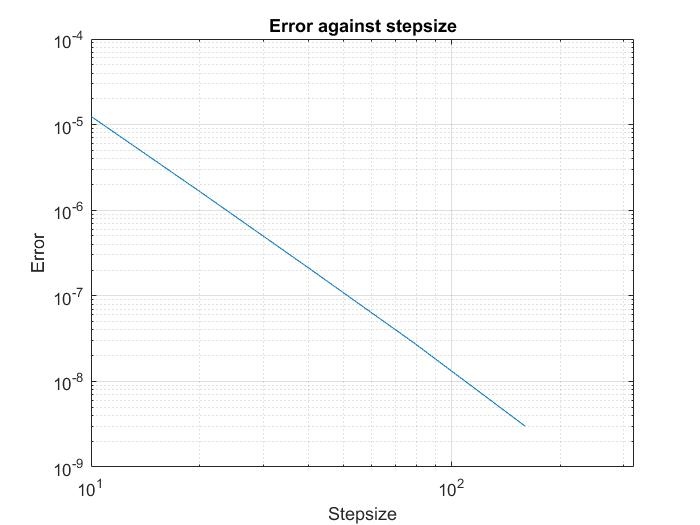
\includegraphics[width=0.45\textwidth,center]{1}
\end{figure}
\newpage

\section*{Problem description}
In this exercise, the following PDE shall be solved.
\begin{equation}
\rho C_p \frac{\partial T}{\partial t} = k\frac{\partial^2 T}{\partial x^2}, \quad t>0, \quad 0<x<L
\end{equation}
With the boundary condition:
\begin{equation}
T\left(0,t\right) = 
\begin{cases} 
T_0 \quad \textrm{if} \quad 0\leq t \leq t_p \\
0 \quad \textrm{if} \quad t \geq t_p
\end{cases}, \qquad \frac{\partial T}{\partial x} \left(L, t\right) = 0
\end{equation}
and the initial condition:
\begin{equation}
T\left(x,0\right) = \begin{cases}
T_0 \quad \textrm{if} \quad x = 0 \\
0 \quad \textrm{if} \quad 0 < x \leq L
\end{cases}
\end{equation}
Here , $\rho$ is the density $\left[kg/m^3\right]$, $C_p$ is the heat capacity $\left[J/(kg\cdot C)\right]$, and $k$ is the thermal conductivity $\left[J/(m\cdot s\cdot C)\right]$. 

\subsection*{1}
If the following parameters are changed, then we can get a dimensionless PDE. 
\begin{equation}
T =T_0 u , \qquad x=L\xi, \qquad t = t_p\tau
\end{equation}
We plug in these new parameters in the equation. Then the following equation can be formulated.
\[
\rho C_p \frac{\partial(T_0 u)}{\partial\tau} \frac{d\tau}{dt} = k \frac{\partial^2(T_0 u)}{\partial(L\xi)^2} \Rightarrow
\]
\[
\rho C_p T_0 \frac{\partial u}{\partial \tau}\cdot \frac{1}{t_p} = k T_0 \frac{\partial^2 u}{\partial \xi^2}\cdot\frac{1}{\frac{\partial(L\xi)^2}{\partial \xi^2}} \Rightarrow
\]
\[
\frac{\partial u}{\partial \tau} = \frac{k\tau_p}{L^2 \rho C_p} \cdot \frac{\partial^2 u}{\partial \xi^2} \Rightarrow
\]
\begin{equation}
\frac{\partial u}{\partial \tau} =  a \frac{\partial^2 u}{\partial \xi^2} \textrm{ where } a = \frac{k\tau_p}{L^2 \rho C_p}
\end{equation}

The boundary conditions can be transformed easily to the following. 
\begin{equation}
u(0,\tau) = \begin{cases} 
1 & \textrm{ if } 0\leq \tau \leq 1 \\
0 & \textrm{ if } 1 < \tau 
\end{cases} 
\textrm{, }\qquad \frac{\partial u}{\partial \xi}(1,\tau) = 0
\end{equation}
and the initial condition become:
\begin{equation}
u\left(\xi,0\right) = \begin{cases}
1 \quad \textrm{if} \quad \xi = 0 \\
0 \quad \textrm{if} \quad 0 < \xi \leq 1 \end{cases}
\end{equation}

Since we got $a = \frac{k\tau_p}{L^2 \rho C_p}$, a dimensions analysis can be done on $a$. 
\[
[a] = \left[\frac{\frac{J}{m\cdot s\cdot C}\cdot s}{m^2\cdot \frac{kg}{m^3}\cdot \frac{J}{kg\cdot c}}\right] = [1] = 1
\]
Thus $a$ is a dimensionless constant which from now on we assume to be $1$.

\subsection*{2}
To compute the value of the function, a discretization is needed for each discretized time step. The second derivative can be computed by central difference method. Let discrete the definition domain of $u$ into $N$ uniform cells each with length $h$. Then we shall have $u_0 \Rightarrow \xi = 0 = \xi_0$ and $u_N \Rightarrow \xi = 1 = \xi_N$. Thus for the $i$:th cell $u_i = u(\xi_i)$ where $i$ goes from 1 to N: 
\[
\Delta u_i = \frac{u_{i+1}-2u_i+u_{i-1}}{h^2} = \frac{d u_i}{d t}
\]
However, we need to add the boundary condition into this formula. Let $f(\tau)=\begin{cases}
1 \quad \textrm{if} \quad \xi = 0 \\
0 \quad \textrm{if} \quad 0 < \xi \leq 1 \end{cases}$. Then $u_0(\tau) = u(0,\tau) = f(\tau)$. When $i=1$, we shall have that:
\[
\Delta u_1 = \frac{u_{2}-2u_1+u_{0}}{h^2} = \frac{u_{2}-2u_1}{h^2} + \frac{f(\tau)}{h^2}
\]
On the other end, we have $\frac{\partial u}{\partial \xi} = \frac{u_{N+1}-u_{N-1}}{2h} = 0 \Rightarrow u_{N+1} = u_{N-1}$. So when $i=N$: 
\[
\Delta u_i = \frac{u_{N+1}-2u_N+u_{N-1}}{h^2} =  \frac{-2u_N+2u_{N-1}}{h^2} 
\]

Thus for each time, we can derive the following ODE: 
\begin{equation}
\frac{d\vec{u}}{dt} = \frac{1}{h^2} 
\begin{pmatrix}
  -2 &  1  &  0  &  0  &  0  & \cdots & 0 \\
  1  & -2  &  1  &  0  &  0  & \cdots & 0\\
  0  &  1  & -2  &  1  &  0  & \cdots & 0\\
  \vdots  & \vdots  & \vdots & \vdots & \vdots & \vdots & \vdots \\
  0 & \cdots & 0 & 0 & 1 & -2 & 1 \\
  0 & \cdots & 0 & 0 & 0 &  2 & -2 \\
 \end{pmatrix}
 \begin{pmatrix}
 u_1 \\ u_2 \\ u_3 \\ \vdots \\ u_{N-1} \\ u_N
 \end{pmatrix}
 +
 \begin{pmatrix}
 f(\tau)/h^2 \\ 0 \\ 0 \\ \vdots \\ 0 \\ 0
 \end{pmatrix} = A\vec{u} + \vec{b}
\end{equation}

































\subsection*{3}

The ODE system in step 2 is discretized in time with step size $\Delta t$. By Euler's explicit method, one obtains a new value of the vector \textbf{u} by setting

\begin{equation}
u_{t_i}=u_{t_{i-1}}+\frac{du_{t_i}}{dt}\Delta t
\end{equation}

with $\Delta t =t_i-t_{i-1}$ and $d\bm{u}_{t_i}= Au_{t_i}+\bm{b}(t_i)$ and initial conditions given in C5.

The solution will be stable if and only if $\frac{\Delta t}{h^2}\leq\frac{1}{2}$. Below, two solutions are shown when the condition holds and when it does not.



\begin{figure}[h]
\centering
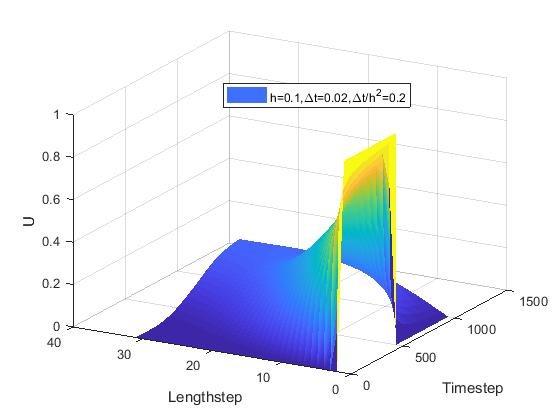
\includegraphics[width=\textwidth,center]{p3f1}
\caption{Stable numerical solution for the PDE.}
\end{figure}
 
 \begin{figure}[h]
\centering
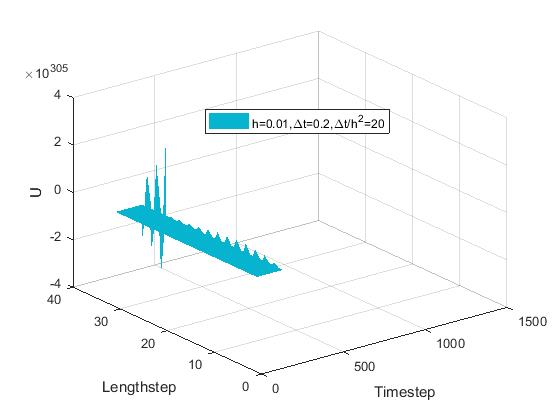
\includegraphics[width=\textwidth,center]{p3f2}
\caption{Unstable solution for the PDE.}
\end{figure}
 



\section*{4}

In this part, Matlabs built in functions ode23 and ode23s are used instead of eulers explicit method in part 3 to solve the ODE obtained in part 2.

The CPU-computing time along with the number of time steps and the maximum step size is summarized in table X.


\begin{table}[h]
\begin{center}
\begin{tabular}{ | c | c | c |c|}
\hline
   & Time Steps    & CPU - Time      & $\Delta t_{max}$  \\ \hline
N  &  ode23 ode23s &  ode23   ode23s &   ode23 ode23s  \\ \hline
10 &   501   466   &  0.0936  0.2652 &  0.0144  0.0198 \\ \hline 20 &   500   460   &  0.0312  0.3432 &  0.0117  0.0317 \\ \hline
40 &   499   461   &  0.1092 4.5864 &  0.0121  0.0278 \\ \hline
\end{tabular}
\end{center}
\label{Statistics for comparison between ode23 and ode23s}
\end{table}
Note the inefficiency of ode23s as the step size increases to 40.



\section*{5}


The function ode and ode23s in Matlab uses the Jacobian of the function $f(\tau,u)=A\textbf{u}+\textbf{b}(\tau)$ when solving the ODE $\frac{du}{dt}=f(\tau,u)$.

Unless specified, the Jacobian is estimated numerically element wise. This process can be made more efficient if one can provide information about the Jacobian to Matlab.


By using the option "Jpattern" one can specify the pattern in the Jacobian by inputting a matrix with ones as elements where the Jacobian would be non-zero. In the case of the ODE in equation (8) the Jacobian will be of the same form as A since u is a linear in its elements and b does not depend on u. 

So if the ode23 and ode23s is called with the Jpattern option using the matrix 
\begin{equation}
S=
\begin{pmatrix}
  1 &  1  &  0  &  0  &  0  & \cdots & 0 \\
  1  & 1  &  1  &  0  &  0  & \cdots & 0 \\
  0  &  1  & 1  &  1  &  0  & \cdots & 0\\
  \vdots  & \vdots  & \vdots & \vdots & \vdots & \vdots  & \vdots  \\
  0 & \cdots & 0 & 0 & 1 & 1 & 1 \\
  0 & \cdots & 0 & 0 & 0 &  1 &  1\\
 \end{pmatrix}
\end{equation}

one obtains the following statistics:

\begin{table}[h]
\begin{center}
\begin{tabular}{ | c | c | c |c|}
\hline
   & Time Steps    & CPU - Time      & $\Delta t_{max}$  \\ \hline
N  &  ode23 ode23s &  ode23   ode23s &   ode23 ode23s  \\ \hline
10 &   501   460   &  0.0468 0.1560  &  0.0144  0.0201 \\ \hline 20 &   500   453   &  0.0312  0.1404 &  0.0117  0.0318 \\ \hline
40 &   499   462   &  0.0624 0.3744 &  0.0121  0.0278 \\ \hline
\end{tabular}
\end{center}
\label{Statistics for comparison between ode23 and ode23s}
\end{table}

And it is evident that by specifying the form of the Jacobian the CPU Time has been reduced drastically.




Another option is to Explicitly specify the Jacobian which is easily done in this case since it simply equals the matrix $\textbf{A}/h^2$ in equation (8).

When this is provided in ode23 and ode23s the following result is obtained.

\begin{table}[h]
\begin{center}
\begin{tabular}{ | c | c | c |c|}
\hline
   & Time Steps    & CPU - Time      & $\Delta t_{max}$  \\ \hline
N  &  ode23 ode23s &  ode23   ode23s &   ode23 ode23s  \\ \hline
10 &   501   453   &  0.0468  0.0936 &  0.0144  0.0200 \\ \hline 20 &   500   1168   &  0.2028  0.0117 &  0.0125  0.0317 \\ \hline
40 &   499   3408   &  0.0468 0.7488 &  0.0121  0.00364 \\ \hline
\end{tabular}
\end{center}
\label{Statistics for comparison between ode23 and ode23s}
\end{table}












































\section*{6}
The 3D plot is showed in the section 3 above as figure 1. The plot of $u(\tau,\xi)$ for $\tau = 0.5, 1.0, 1.5, 2.0$ is showed below. 

\begin{figure}[h]
\centering
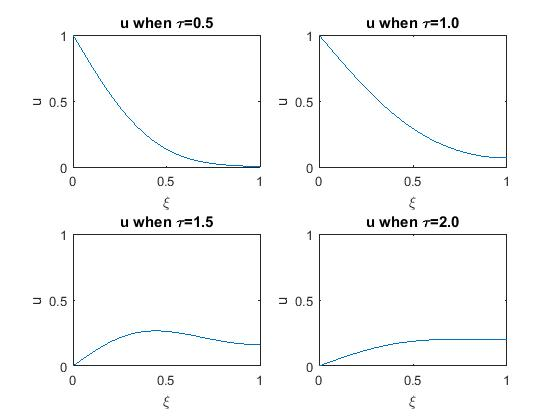
\includegraphics[width=\textwidth,center]{p6f1}
\caption{Numerical solutions corresponding to different $\tau$}
\end{figure}

Conclusions we can draw from this lab are the following. 
If we want to do an efficient numerical computations for parabolic problems, a non-stiff ODE method should be used. The jacobian of the ODE system has a sparse structure similar to the A matrix. Thus a linear equation solver for sparse matrices shall be used to maximize the performance. 

\end{document}










































%%LAB 4 Carl & Yue
%%Numerical Solution to a heat equation
clear all,close all, clc

%Defining matrices
%% Part 1-4


for h=[0.1 0.01] 
N=30;
dt=0.002;
A=[];
for i = 2:N-1
A(i,i)=-2;
A(i,i+1)=1;
A(i,i-1)=1;
end

A(1,2)=1;
A(1,1)=-2;
A(N,N)=-2;
A(N,N-1)=2;

A=1/h^2*sparse(A);

b=zeros(1,N)';
u=zeros(1,N)';
U = [1; u];

for t=0:dt:2
   
    %BC
if t> 1
    func = 0;
else
    func = 1;
end 

b(1)=func/h^2;

du=A*u+b;

u=u+du*dt;

if t<=1
    U = [U, [1; u]];
else
    U = [U, [0; u]];
end
if abs(h-0.1)<eps
    if  abs(t-0)< eps
       subplot(2,2,1)
       plot(0:1/N:1, [1; u])
       title('u when \tau=0.5')
       xlabel('\xi')
       ylabel('u')
       xlim([0 1])
       ylim([0 1])
    end
    
    if  abs(t-1)< eps
       subplot(2,2,2)
       plot(0:1/N:1, [1; u])
       title('u when \tau=1.0')
       xlabel('\xi')
       ylabel('u')
       xlim([0 1])
       ylim([0 1])
    end
    
    if  abs(t-1.5)< eps
       subplot(2,2,3)
       plot(0:1/N:1, [0; u])
       title('u when \tau=1.5')
       xlabel('\xi')
       ylabel('u')
       xlim([0 1])
       ylim([0 1])
    end
    
    if  abs(t-2)< eps
       subplot(2,2,4)
       plot(0:1/N:1, [0; u])
       title('u when \tau=2.0')
       xlabel('\xi')
       ylabel('u')
       xlim([0 1])
       ylim([0 1])
    end
end
end
time=0:dt:10;
figure

%Adding the BC point

% U= leng

surf(U,'edgecolor','none')
legend(['h=' num2str(h) ',' '\Deltat=' num2str(dt/h) ',' '\Deltat/h^2=' num2str(dt/(h^2))])
xlabel('Timestep')
ylabel('Lengthstep')
zlabel('U')

end

%% Part 4
figure
A=[];
k=1;
for N=[10 20 40]


odefuncN = @(t,u) odefunc(t,u,N);

time = cputime;
[t,u]=ode23(odefuncN,[0 2],zeros(1,N)',odeset('RelTol',1e-6));
e(k) = cputime-time;
 
times1 =cputime;
[ts,us]=ode23s(odefuncN,[0 2],zeros(1,N)',odeset('RelTol',1e-6));
es(k) = cputime-times1;

timev(k)=length(t);
maxdifft(k)=max(diff(t));

timevs(k)=length(ts);
maxdiffts(k)=max(diff(ts));

k=k+1;


surf(us','edgecolor','none')
figure
surf(u','edgecolor','none')
end
A(:,1)=timev;
A(:,2)=timevs;
A(:,3)=e;
A(:,4)=es;
A(:,5)=maxdifft;
A(:,6)=maxdiffts;
format short
A1=A




%% Part 5

%Testing JPATTERN OPTION WITH S
A=[];
k=1;
for N=[10 20 40]

    S=[];
for i = 2:N-1
S(i,i)=1;
S(i,i+1)=1;
S(i,i-1)=1;
end

S(1,2)=1;
S(1,1)=1;
S(N,N)=1;
S(N,N-1)=1;



odefuncN = @(t,u) odefunc(t,u,N);

time = cputime;
[t,u]=ode23(odefuncN,[0 2],zeros(1,N)',odeset('RelTol',1e-6,'Jpattern',S));
e(k) = cputime-time;
 
times1 =cputime;
[ts,us]=ode23s(odefuncN,[0 2],zeros(1,N)',odeset('RelTol',1e-6,'Jpattern',S));
es(k) = cputime-times1;

timev(k)=length(t);
maxdifft(k)=max(diff(t));

timevs(k)=length(ts);
maxdiffts(k)=max(diff(ts));

k=k+1;



end
A(:,1)=timev;
A(:,2)=timevs;
A(:,3)=e;
A(:,4)=es;
A(:,5)=maxdifft;
A(:,6)=maxdiffts;
A2=A

% EXPLICITLY SPECIFYING THE JACOBIAN

A=[];
k=1;
for N=[10 20 40]

 J=[];

for i = 2:N-1
J(i,i)=-2;
J(i,i+1)=1;
J(i,i-1)=1;
end

J(1,2)=1;
J(1,1)=-2;
J(N,N)=-2;
J(N,N-1)=2;
J=1/(1/N)^2*sparse(J);



odefuncN = @(t,u) odefunc(t,u,N);

time = cputime;
[t,u]=ode23(odefuncN,[0 2],zeros(1,N)',odeset('RelTol',1e-6,'Jacobian',J));
e(k) = cputime-time;
 
times1 =cputime;
[ts,us]=ode23s(odefuncN,[0 2],zeros(1,N)',odeset('RelTol',1e-6,'Jacobian',J));
es(k) = cputime-times1;

timev(k)=length(t);
maxdifft(k)=max(diff(t));

timevs(k)=length(ts);
maxdiffts(k)=max(diff(ts));

k=k+1;

surf(us','edgecolor','none')
figure
surf(u','edgecolor','none')

end
A(:,1)=timev;
A(:,2)=timevs;
A(:,3)=e;
A(:,4)=es;
A(:,5)=maxdifft;
A(:,6)=maxdiffts;
format long
A3=A




